% Useful links
% List of math symbols: https://oeis.org/wiki/List_of_LaTeX_mathematical_symbols
% Font sizes: http://www.sascha-frank.com/latex-font-size.html

\documentclass[10pt,fleqn]{article}

\usepackage{algorithm}
\usepackage[noend]{algpseudocode}
\usepackage{amsfonts}
\usepackage{amsmath}
\usepackage{amssymb}
\usepackage{amsthm}
\usepackage[english, ngerman]{babel}
\usepackage{cancel}
\usepackage{enumitem}
\usepackage{fullpage}
\usepackage{hyperref}
\usepackage{latexsym}
\usepackage{listings}
\usepackage{mathtools}
\usepackage{nccmath}
\usepackage{polynom}
\usepackage{subcaption}
\usepackage{tabularx}
\usepackage{tikz}
\usetikzlibrary{calc, positioning, shapes}
\usepackage{wasysym}
\usepackage{wrapfig}
\usepackage{xcolor}

% https://tex.stackexchange.com/questions/89166/centering-in-tabularx-and-x-columns
% and https://tex.stackexchange.com/questions/257128/how-does-the-newcolumntype-command-work
% Combines c + X in tabularx environments.
% Inserts centering command after the entry in the cell to center it.
\newcolumntype{Y}{>{\centering\arraybackslash}X}

\hypersetup{
    colorlinks   = true,
    urlcolor     = blue,
    linkcolor    = blue,
    citecolor    = red
}

\setlength{\parindent}{0pt}

% I do not really like the plain style
%\theoremstyle{plain}
\theoremstyle{definition}
\newtheorem{definition}{Definition}
\newtheorem{theorem}{Theorem}
\newtheorem{proposition}{Proposition}
\newtheorem{lemma}[theorem]{Lemma}
\newtheorem{corollary}{Corollary}
\newtheorem{fact}{Fact}
\theoremstyle{remark}
\newtheorem{remark}{Remark}

\newcommand{\Task}{x}
\newcommand{\Authors}{valentinpi}
\newcommand{\task}[1]{\item{\bfseries #1}}

\newcommand{\pclass}{\text{P}}
\newcommand{\npclass}{\text{NP}}
\newcommand{\pathprob}{\text{PATH}}
\newcommand{\relprimeprob}{\text{RELPRIME}}
\newcommand{\cflclass}{\text{CFL}}
\newcommand{\hampathprob}{\text{HAMPATH}}
\newcommand{\compositesprob}{\text{COMPOSITES}}
\newcommand{\cliqueprob}{\text{CLIQUE}}
\newcommand{\subsetsumprob}{\text{SUBSET-SUM}}
\newcommand{\satprob}{\text{SAT}}
\newcommand{\threesatprob}{\text{3SAT}}
\newcommand{\spaceclass}{\text{SPACE}}
\newcommand{\nspaceclass}{\text{NSPACE}}
\newcommand{\pspaceclass}{\text{PSPACE}}
\newcommand{\npspaceclass}{\text{NPSPACE}}
\newcommand{\exptimeclass}{\text{EXPTIME}}
\newcommand{\tqbfprob}{\text{TQBF}}
\newcommand{\formulagameprob}{\text{FORMULA-GAME}}
\newcommand{\ggprob}{\text{GG}}

\newcommand{\lpp}{\left \langle}
\newcommand{\rpp}{\right \rangle}
\newcommand{\enc}[1]{\lpp #1 \rpp}

\DeclareMathOperator{\onot}{\mathcal{O}}
\DeclareMathOperator{\omnot}{\Omega}
\DeclareMathOperator{\thetnot}{\Theta}

\renewcommand{\qedsymbol}{\(\blacksquare\)}

\begin{document}
\pagenumbering{arabic}
\title{
    \vspace*{-12ex}
    \phantom{}\\
    \normalsize Handout\\
    \phantom{}\\
    \large The Class PSPACE and Game Theory\\
    \phantom{}\\
    \normalsize Proseminar Theoretische Informatik WiSe 2020-21\\
    \normalsize Institut für Informatik\\
    \normalsize Freie Universität Berlin
}
\author{\normalsize \Authors}
\date{
    \normalsize 5. Januar 2021\\
    (neueste Version)
    \rule{\textwidth}{0.1pt}
}
\selectlanguage{ngerman}
\maketitle
\selectlanguage{english}
\vspace{-2\baselineskip}
\begin{abstract}
    \noindent This handout presents the complexity class PSPACE. It presents the most important definitions in the context of the language hierarchy after the P and NP presentations. It then presents its applications in the formula game and the geography game.
\end{abstract}

\paragraph*{Space Complexity and the Class PSPACE} One can analyze efficiency in at least three different ways: Time, space, encoding efficiency. Looking at space efficiency leads to the first complexity classes here:
\begin{definition} Let \(f\colon \mathbb{N} \rightarrow \mathbb{R}^+\) be a function. The complexity classes \emph{SPACE} and \emph{NSPACE} of \(f\) are:
\begin{align*}
    &\spaceclass(f(n)) \coloneqq \{ \; L \mid L \text{ is decided by a deterministic turing machine using } \mathcal{O}(f(n)) \text{ space} \; \}\\
    &\nspaceclass(f(n)) \coloneqq \{ \; L \mid L \text{ is decided by a nondeterministic turing machine using } \mathcal{O}(f(n)) \text{ space} \; \}
\end{align*}
\end{definition}
Instead of time, to analyze whether problems are in these classes, one has to consider how much space, i.e. memory or tape cells of a TM, an algorithm uses. As you can see, these definitions are analogous to the ones for TIME and NTIME.
\begin{definition} In analogy to the classes P and NP, \emph{PSPACE} and \emph{NPSPACE} are defined as:
    \[
        \pspaceclass \coloneqq \bigcup_{k \in \mathbb{N}} \spaceclass(n^k) \qquad
        \npspaceclass \coloneqq \bigcup_{k \in \mathbb{N}} \nspaceclass(n^k)
    \]
\end{definition}
One very important and surprising result of complexity theory is the following: The researcher Savitch showed that any nondeterministic polynomial space bounded machine can be simulated by such a deterministic machine in about quadratic more space. Since \(\pspaceclass \subseteq \npspaceclass\) per definition:
\begin{fact}[Corollary from Savitchs Theorem]
\(
    \pspaceclass = \npspaceclass
\)
\end{fact}
As in NP-completeness, completeness is also defined for PSPACE-Problems:
\begin{definition} A language \(B\) is \emph{PSPACE-complete}, if:
    \begin{enumerate}
        \item \(B \in \pspaceclass\)
        \item \(A \leq_p B\) for all \(A \in \pspaceclass\), also called \emph{PSPACE-hard}
    \end{enumerate}
\end{definition}
\begin{itemize}
    \item Complete problems exist for many complexity classes, not just NP
    \item \(\leq_p\) denotes \emph{polynomial time reducibility}, not space reducibility. Time is also a bound for the space used, since a machine can not occupy more space than it can move its read/write head.
\end{itemize}
\begin{fact} The following holds:
    \begin{ceqn}
        \[
            \pclass \subseteq \npclass \subseteq \pspaceclass = \npspaceclass \subseteq \exptimeclass \coloneqq \bigcup_{k \in \mathbb{N}} \text{TIME}\left(2^{n^k}\right), \; \pclass \neq \exptimeclass
        \]
    \end{ceqn}
\end{fact}

\newpage

\paragraph*{Quantified Boolean Formulas} The following is a generalization of the SAT-Problem with \emph{quantifiers}.

Some important terms:
\begin{itemize}
    \item Any boolean formula can be put into \emph{prenex normal form}: Quantifiers appear first and then the boolean formula without quantifiers. General form: \(\text{Q}_1x_1\text{Q}_2x_2...\text{Q}_nx_n\colon\phi\) with \(\text{Q}_1,...,\text{Q}_n \in \{\forall,\exists\}\)
    
    An example:
    \begin{ceqn}
    \[
        \phi = \underbrace{\exists x_1 \forall x_2, x_3\colon}_{\text{bounded variables}} \underbrace{(x_1 \lor x_2) \lor x_3}_{\text{scope}} \text{ is in prenex normal form}
    \]
    \end{ceqn}
    \item Such a formula is \emph{fully quantified}, if each variable of the formula appears in the scope of a quantifier, like in the formula above.
    \item Fully quantified formulas are either true or false, since they are statements themselves.
\end{itemize}
This generalization of SAT is called \emph{TBQF}: \(
        \tqbfprob \coloneqq \{\; \enc{\phi} \mid \phi \text{ is a true fully quantified boolean formula}\;\}
    \)
\begin{theorem}
    \(
        \tqbfprob
    \) is PSPACE-complete.
\end{theorem}
\begin{proof} \(\tqbfprob \in \pspaceclass\) can be shown by giving a recursive algorithm. Since all the quantifiers are first and the variables can only get assigned to a finite number of values - true or false -, our algorithm can check all possible combinations of variable assignments:
    \begin{description}
        \item[Input:] \(\enc{\phi}\), where \(\phi\) is a fully quantified boolean formula.
        \item[Function:] \phantom{}
            \begin{algorithmic}[1]
                \If{\(\phi = \psi\) has no quantifiers}
                    \State \(\psi\) has no quantifiers, only constants. Evaluate \(\psi\), accept or reject depending on result.
                \ElsIf{\(\phi\) has form \(\exists x\colon \psi\) (\(\psi\) is remaining term)}
                    \State Recursive call on \(\psi\), once with \(x\) substituted with false, once substituted with true.
                    \State If either accepts, accept. Otherwise, reject.
                \Else{ \(\phi\) has form \(\forall x\colon \psi\)}
                    \State Recursive call on \(\psi\), once with \(x\) substituted with false, once substituted with true.
                    \State If both accept, accept. Otherwise, reject.
                \EndIf
            \end{algorithmic}
    \end{description}
    The additional space the algorithm uses is limited by the number of recursions. Those can be at most \(n\) with \(n\) being the number of variables that appear in the formula. Therefore the algorithm runs in \(\mathcal{O}(n)\) space, which is polynomial.\\

    For the PSPACE-hardness we will only consider the proof idea here. The first idea would be, since this is a generalization of the SAT-problem, to consider the proof from Cook-Levin and simulate execution of the polynomial space bounded TM of some \(A \in \pspaceclass\) using a fully quantified boolean formula.\\
    
    However, such a TM for \(A\) could run in exponential time! So the reduction may produce a simulation, the quantified boolean formula, that is of exponential size. A polynomial time reduction can not produce an exponential sized result.

    Using techniques from the Theorem of Savitch, one can use universal quantifiers \(\forall\) to divide the formula for the TM into subformulas. So the idea is to use another technique to make the previous formula much smaller.
\end{proof}

To prove PSPACE-completeness for more problems using TQBF, one can use this corollary from NP-completeness:
\begin{corollary}
    If \(B\) is PSPACE-complete and \(B \leq_p C\) for \(C \in \pspaceclass\), then \(C\) is PSPACE-complete.
\end{corollary}

\newpage

\paragraph*{Game Theory and the FORMULA-GAME Problem} Here, a \emph{game} is a competition between two opposing players, in which both want to achieve some goal under specific rules. There are casual games like chess and go, but also more serious games, which model war or societal conflict.\\

Fully quantified formulas decode games. One may recall this analogy from the logic lectures. Player A (\emph{All}) and player E (\emph{Exists}) take turns choosing assignments for the universally (\(\forall\)) and existentially (\(\exists\)) quantified variables of such a formula \(\phi\) from left to right. If the formula evaluates to false, A wins. Otherwise, E wins. We call this game the \emph{formula game}. One of these players has a \emph{winning strategy}, if assignments can be chosen so that that player wins no matter what is chosen afterwards.\\

\textbf{Example:} \(\exists x_1 \forall x_2, x_3\colon x_1 \lor x_2 \land x_3\) - If E chooses \(x_1 = 1\), the formula will evaluate to true and E wins, no matter what A chooses.\\

We define the following problem:
\begin{ceqn}
    \[
        \formulagameprob \coloneqq \{ \; \enc{\phi} \mid \text{Player E has a winning strategy in the formula game on } \phi \; \}
    \]
\end{ceqn}

The following corollary shows that, even though the problems TQBF and FORMULA-GAME are seemingly different - one is about fully quantified boolean formulas and one is about gaming - they are actually the same.

\begin{corollary} \(\formulagameprob = \tqbfprob\) and \(\formulagameprob\) is PSPACE-complete.
\end{corollary}
\emph{Reason.} \((\subseteq)\) If player E has a winning strategy for the formula game associated with a fully quantified boolean formula \(\phi\), then, no matter how A chooses the variables bound to universal quantifiers to be assigned, E will win with the game with the strategy. Similarly, these assignments correspond to variable assignments for the existential quantifiers, and the fact that A can not prevent the loss means that the statement is true for any assignment of the universal quantifiers. Therefore, \(\phi\) must be true, if E has such a strategy.

\((\supseteq)\) Similarly, if \(\phi\) is a true formula, player E can win by using the variable assignments for variables bound to existential quantifiers as the winning strategy. The problems are identical.

\paragraph*{The Game Geography and the GG Problem} Another game is \emph{geography}. In geography, two players I and II take turns naming cities from all around the world. The first city is chosen in advance. Player I must then choose a city that starts with the last letter of the first city, no repetitions allowed. Then player II chooses a next city and so on. If one player runs out of city names, the other player wins.\\

\textbf{Example:} A game starts with Paris. Player I chooses St. Malo, since it starts with S. Player II chooses Orleans, then I chooses Strasbourg. Continue with Grenoble and Epernay. Player II, in this case, does not know any city starting with Y, so I has won this game.

\begin{figure}[!hbtp]
    \centering
    \begin{subfigure}{0.34\linewidth}
        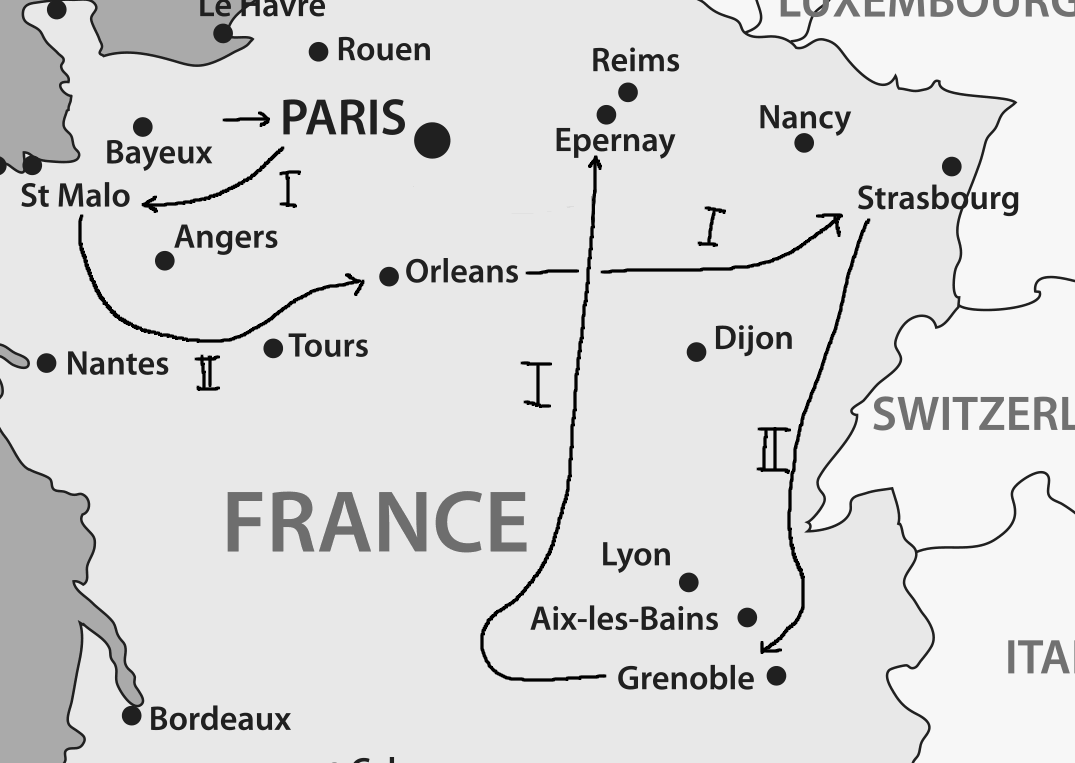
\includegraphics[width=\linewidth]{img/map-of-france-geography.png}
    \end{subfigure}
    \begin{subfigure}{0.34\linewidth}
        \resizebox{\linewidth}{!}{%
            \begin{tikzpicture}[
                ->,
                >=stealth,
                every node/.style={draw, ellipse}
            ]
                \scriptsize
                \node (0) at (0, 0) {Paris};
                \node (1) at (-2, -1) {St. Malo};
                \node (2) at (1, -1.5) {Orleans};
                \node (3) at (4, -1) {Strasbourg};
                \node (4) at (3, -3) {Grenoble};
                \node (5) at (2, 0) {Epernay};
                \path (-1, 0) edge (0)
                (0) edge[bend left=25] node[draw=none, right] {I} (1)
                (1) edge node[draw=none, below] {II} (2)
                (2) edge node[draw=none, above right] {I} (3)
                (3) edge node[draw=none, above left] {II} (4)
                (4) edge node[draw=none, below left] {I} (5);
            \end{tikzpicture}%
        }
    \end{subfigure}
    \caption[A game of geography on the map of France.]{A game of geography on the map of France.\footnotemark}
\end{figure}
\footnotetext{\url{https://i.pinimg.com/originals/f6/e6/c5/f6e6c586d8b62dc6e66fa2e85dad2ad8.png}, last accessed: 27.12.2020, 22:30}

This example only used French cities, but in geography one generally talks about cities from all around the world. The cities named induce a directed graph over the map of the world.

One can generalize this problem for any directed graph with a start node, called \emph{generalized geography} (GG):
\begin{ceqn}
    \[
        \ggprob \coloneqq \{\; \enc{G, s} \mid \text{Player I has a winning strategy for the GG game played on }G\text{, starting from } s \;\}
    \]
\end{ceqn}

\begin{theorem}
    \(\ggprob\) is PSPACE-complete.
\end{theorem}
\begin{proof}
    The proof uses the Corollary 1. First, show that \(\ggprob \in \pspaceclass\), then show \(\formulagameprob \leq_p \ggprob\). The following algorithm decides GG:
    \begin{description}
        \item[Input:] \(\enc{G, s}\), where \(G\) is a directed graph and \(s\) a node from \(G\).
        \item[Function:] \phantom{}
            \begin{algorithmic}[1]
                \If{\(\deg{s} = 0\) (the degree \(\deg\) is the number of neighbors of a node)}
                    \State Reject, since Player I instantly looses.
                \EndIf
                \State Remove \(s\) and its edges from \(G\) for a new graph \(G'\).
                \State For the outgoing neighbors of \(s\), \(s_1, ..., s_k\), do a recursive call on \(\enc{G', s_i}\), \(i \in \{1,...,k\}\).
                \State If all accept, reject, since the current player would lose. Otherwise, accept, since the opposing player gets stuck.
            \end{algorithmic}
    \end{description}
    During execution, the algorithm implicitely switches perspective from player I to II and vice versa when it recurses. When we reject, the current player loses due to the first if-statement. When we accept, we win.
    
    About the complexity: The machine only needs to store each node when it recurses into the neighbors. Therefore the space complexity is \(\mathcal{O}(n)\) with \(n\) being the number of nodes, which is polynomial.\\

    \begin{minipage}{0.5\linewidth}
        Now for the second statement. Let
        \[\phi = \exists x_1 \forall x_2 \exists x_3 ... \exists x_n\colon \psi\]
        be a formula game with \(\psi\) in conjunctive normal form. The quantifiers start and end with existential ones and strictly alternate. If not, insert quantifiers for dummy variables, which are not used in \(\psi\).

        An example for the constructed geography game is demonstrated on the right side. For each variable, a diamond-shaped structure is introduced, with which the players implicitely assign truth values to variables. Using dummy nodes between each diamond, the players take their turns choosing. When \(x_n\) has been assigned by player I, an assignment of all variables was made. Player II reaches the node \(c\), which represents a choice between the clauses of the formula.

        For each clause and each literal, we introduce nodes. \((\Rightarrow)\) If the player I has a winning strategy for \(\phi\), player II can choose any clause of \(c_1, c_2, ..., c_m\). Player I then must choose one true literal from the clause, which exists, since the formula is satisfied. The literal only has an edge back to the choice made, but it has already been made, since the literal is true. Player II is stuck and player I wins. If player II has a winning strategy, one node was not visited and II can choose the literal for it. Player I would then get stuck. \((\Leftarrow)\) The assignment made directly corresponds to a winning strategy in the formula game, which completes the reduction.
    \end{minipage}
    \begin{minipage}{0.5\linewidth}
        \begin{tikzpicture}[
            every node/.style={draw, circle, minimum size=5mm, inner sep=0mm},
            >=stealth,
            scale=0.9
        ]
            \node (0) at (0, 0) {\(s\)};
            \node[below left of=0] (10) {};
            \node[below right of=0] (11) {};
            \node[draw=none, left of=10] {\(x_1\)};
            \node[below right of=10] (2) {};
            \node[below of=2] (3) {};
            \node[below left of=3] (40) {};
            \node[below right of=3] (41) {};
            \node[draw=none, left of=40] {\(x_2\)};
            \node[below right of=40] (5) {};
            \node[below of=5] (6) {};
            \node[draw=none,below of=6] (7) {...};
            \node[below of=7] (8) {};
            \node[below left of=8] (90) {};
            \node[below right of=8] (91) {};
            \node[draw=none, left of=90] {\(x_n\)};
            \node[below right of=90] (100) {};
            \node (c) at (6, -4) {\(c\)};
            \node (c1) at (4, -1) {\(c_1\)};
            \node (c2) at (4, -3) {\(c_2\)};
            \node[draw=none] (etc) at (4, -5) {...};
            \node (cm) at (4, -7) {\(c_m\)};
            \node (110) at (3, -0.33) {\(x_1\)};
            \node (111) at (3, -1) {\(\overline{x_2}\)};
            \node (112) at (3, -1.66) {\(x_3\)};
            \node (120) at (3, -2.33) {\(\overline{x_1}\)};
            \node (121) at (3, -3) {\(x_2\)};
            \node (122) at (3, -3.66) {};
            \node (130) at (3, -6.33) {};
            \node (131) at (3, -7) {};
            \node (132) at (3, -7.66) {};
            \path[->, draw]
            (0) edge node[above left, draw=none] {\scriptsize true} (10)
            (0) edge node[above right, draw=none] {\scriptsize false} (11)
            (10) edge (2)
            (11) edge (2)
            (2) edge (3)
            (3) edge (40)
            (3) edge (41)
            (40) edge (5)
            (41) edge (5)
            (5) edge (6)
            (6) edge (7)
            (7) edge (8)
            (8) edge (90)
            (8) edge (91)
            (90) edge (100)
            (91) edge (100)
            (100) edge[bend right=60] (c)
            (c) edge (c1)
            (c) edge (c2)
            (c) edge (cm)
            (c1) edge (110)
            (c1) edge (111)
            (c1) edge (112)
            (c2) edge (120)
            (c2) edge (121)
            (c2) edge (122)
            (cm) edge (130)
            (cm) edge (131)
            (cm) edge (132)
            (110) edge[bend right=10] (10)
            (111) edge (41)
            (120) edge (11)
            (121) edge[bend left=25] (40)
            ;
        \end{tikzpicture}
    \end{minipage}
\end{proof}

\newpage

\paragraph*{Another New Landscape} With the introduction of PSPACE, NPSPACE but also EXPTIME the landscape has become larger. Assuming the relations are proper (real subsets, \(\pclass \neq \npclass\), etc.), from Fact 2 one gets:
\begin{figure}[!hbtp]
    \large
    \centering
    \begin{tikzpicture}[
        semithick,
        scale=0.9
    ]
        \draw (-4.5, -1.5) rectangle (6.5, 6.5);
        \node at (-3, 5.75) {EXPTIME};
        \draw (0, 0) ellipse (0.5cm and 0.5cm);
        \node at (0, 0) {P};
        \draw (0.5, 0.25) ellipse (1.5cm and 1cm);
        \node at (1, 0.5) {NP};
        \node at (1, 5) {\(\pspaceclass = \npspaceclass\)};
        \draw (1, 2.5) ellipse (5cm and 3.5cm);
        \node at (1, 3.5) {\normalsize PSPACE-complete};
        \node at (-0.5, 2) {\normalsize \(\ggprob\)};
        \node at (2, 2.5) {\normalsize \(\begin{matrix}
            &\tqbfprob =\\
            &\formulagameprob
        \end{matrix}\)};
        \draw (1.25, 2.75) ellipse (3.15cm and 1.4cm);
    \end{tikzpicture}
\end{figure}

\nocite{*}
\renewcommand{\refname}{\normalsize References}
\bibliography{pspace_handout}
\bibliographystyle{plain}

All the illustrations were made by myself using \emph{LaTex/Tikz}.
\end{document}

% Map of France for geography - Example link: https://i.pinimg.com/originals/f6/e6/c5/f6e6c586d8b62dc6e66fa2e85dad2ad8.png
